\chapter{Background}
\label{background}

In this chapter, we give a brief overview of different \ac{AI} techniques that have been considered for implementing the agent for Quoridor including the minimax algorithm.

\section{Zero-sum game}
A zero-sum game is defined as a game where an advantage to one side means an equal loss to the opponent, resulting in the sum of zero. In zero sum games such as chess, tic-tac-toe, an advantage or a win for a team would mean a disadvantage or a loss for another team. 

An example of a zero sum game is poker where, for example, 5 people buy in with a total of 50 euros each, making the table total of 250 euros. In the end, despite some winners or losers in the game, the total will be distributed among the players. In this game, there will be a zero net gain resulting in a zero sum game.

Similarly, in chess, the evaluation of a given position on the board may be slightly advantageous to white. This will always imply that the position is slightly disadvantageous for the player playing the black pieces. A loss of a rook for black would mean, in some cases, an equivalent loss worth 5 pawns. This would imply an equivalent 5 pawn gain for the opponent playing with the white pieces.


\section{Minimax algorithm}

Minimax algorithm, first proven by John von Neumann in 1928 in his paper \textit{Zur Theorie Der Gesellschaftsspiele}, is a very popular algorithm employed in many decision-making scenarios for e.g., in decision theory, game theory and even philosophy. As suggested by the name minimax, the idea of the algorithm is to minimize the player's loss when the opponent makes a decision that gives the player the maximum loss. This algorithm has been implemented in many two-player zero-sum strategy games such as chess and tic-tac-toe

Mathematically, a minimax algorithm can be defined as the following:
\begin{equation}
    \bar{v}_i = \min_{a_{-i}} \max_{a_{i}} v_i (a_i, a_{-i})
\end{equation}
where,
\begin{align}
    &i = \text{index of the player of interest} \\
    &-i = \text{index of the opponent(s)} \\
    &a_i= \text{action of the player of interest)} \\
    &a_{-i}= \text{action of the opponents)} \\
    &v_i = \text{value function of player i} \\
    &\bar{v}_i = \text{minimax value of the player of interest}
\end{align}

 The value represented by $v_i (a_i, a_{-i})$ defines the  initial set of values or outcomes of the game depending on various actions of the player $i$ and player $-i$. We first marginalize away the set of actions of the the player (e.g., $a_{i}$) from the set of possible outcomes by maximizing the value $v_i$ over the set of every possible action of the player. The implication here is that we are evaluating all the possible actions of the player and selecting the one that maximizes the value function.  We then choose an action $a_{-i}$ from the set of all possible actions of the opponent that minimizes the maximum value function. 

 In a two-player zero sum game, this concept translates to the following interpretation. Given a two person zero sum game with finite actions of the players, there exists a value $V$ such that given an opponent's strategy, the value to the player of interest is $V$. This implies that given the player of interest's chooses the strategy, the opponent's value is $-V$ making the sum zero.

 Below in an example of a minimax algorithm in zero sum game:

 \begin{itemize}
     \item Consider two players A and B.
     \item The players simultaneously choose a number (an integer) between 1 and 5.
     \item The payoff is the difference between the two chosen numbers. For example, if Player A chooses $5$ and player B chooses $1$, Player B has to give $5-1=4$ to Player A.
     \item This can be exemplified with the payoff matrix below:
     \begin{table}[!ht]
         \centering
         \begin{tabular}{|c|c|c|c|c|c|}\hline
               & B chooses 1 & B chooses 2 & B chooses 3 & B chooses 4 & B chooses 5  \\ \hline 
              A chooses 1 & 0 & -1& -2& -3&  -4 \\ \hline
              A chooses 2 & 1 & 0 & -1 & -2 & -3   \\ \hline
              A chooses 3 & 2 & 1 & 0 & -1 & -2  \\ \hline
              A chooses 4 & 3 & 2 & 1 & 0 &  -1 \\ \hline
              A chooses 5 & 4 & 3 & 2 & 1 & 0  \\ \hline
         \end{tabular}
         \caption{Payoff matrix for the described game from the perspective of player A}
         \label{tab:my_label}
     \end{table}
 \end{itemize}
For the $\max_{a_{-i}} v_i (a_i, a_{-i})$ part, the player A first marginalizes away the actions of the opponent $a_{-i}$. This results in the following table:

     \begin{table}[!ht]
         \centering
         \begin{tabular}{|c|c|c|c|c|c|}\hline
               & B chooses 1 & B chooses 2 & B chooses 3 & B chooses 4 & B chooses 5  \\ \hline 
              $\max_{a_i} v_i(a_i, a_{-i})$ & 4 & 3& 2& 1&  0 \\ \hline
         \end{tabular}
         \caption{Marginalied value of the payoff matrix after maximizing over the player's actions}
         \label{tab:my_label}
     \end{table}

 We first marginalize away the set of actions of the player (e.g., $a_{i}$) from the set of possible outcomes by maximizing the value $v_i$ over the set of every possible action of the player. 
 
 We then determine the $\min_{a_{-i}}$ over the set of chosen values and determine that $0$ is the minimum when B chooses 5.

 We determine that for player A, no matter what B chooses, the optimal strategy to maximize the value to the player $i$ is choosing $5$. this is the dominant strategy. This is also known as the dominant strategy when the value of the minimax can be determined only based on player A's actions without depending on the actions of player B. 

 In the above example, the search size is limited. However, in many games such as chess, the size of the search space is too big. In such cases, it would be impossible to perform an exhaustive search on the game space due to limited computational resources. For example, in chess, for every possible action of the player, there are many responses of the opponent. This search space increases even more if we consider the further moves and hence the possibilities of the player and the opponent. In terms of graph, every action of the player can be considered as a node and the action of the opponent can be considered as a child of the node. The further moves of the player and the opponent can be captured by representing the moves as further child nodes.

\begin{figure}
    \centering
    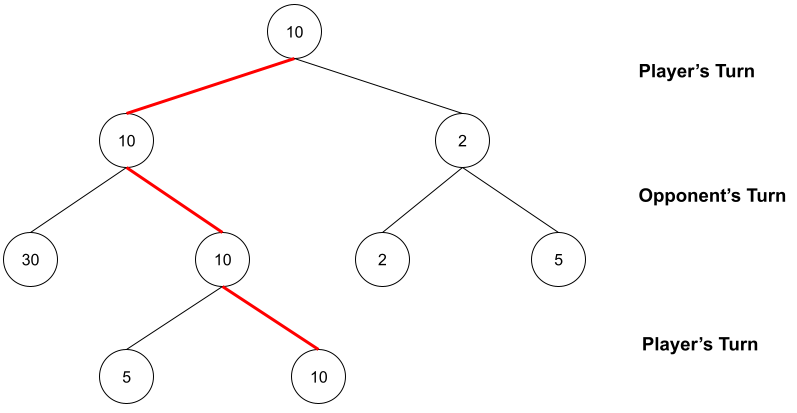
\includegraphics[width=\linewidth]{../img/Minimax1.png}
    \caption{Figure illustrating an exemplary game tree and decision based on minimax algorithm}
    \label{fig:minimax1}
\end{figure}

In Figure \ref{fig:minimax1}, we illustrate an example minimax evaluation and decision selection procedure. The tree in the figure consists of nodes that define either player's or the opponent's actions. For each action, there can be an evaluation where higher evaluation may mean it is favouring the player. For example, an action of the player causing two possible evaluations of 10 and 20 would mean the player would have higher advantage choosing the action leading to evaluation of 20. 

The minimax algorithm first creates a game tree based on all the possible moves of the player and opponent. Then for the leaf node positions, the game position is evaluated and assigned a value. For example, the leaf nodes associated with the branch labelled in red in this graph is assigned values of 5 and 10. In this graph, we do not show further child nodes due for better illustrations, but it can be assumed that the tree has further children nodes. In the game, the player wants to maximize the evaluation on their turn whereas the opponent wants to minimize the evaluation on their turn. The player chooses a move with an evaluation of 10 (maximizing its evaluation) and labels the action as 10. The player then determines that the opponent chooses an action that minimizes the evaluation, choosing an action with evaluation of 10 rather than 30. The player hence labels the parent node as 10 indicating that with best play, the player can achieve an evaluation of 10 from that node. The player then chooses the node with evaluation of 10 when choosing between 10 and 2, maximizing its evaluation and subsequently labels the parent node as 10. The red line shows the path the player determines as optimal leading to a decision choosing the the action labelled with evaluation of 10. 

One way to limit the search space for implementing the minimax algorithm is consider a depth-limited version of the algorithm. In this version, the algorithm only considers a part game tree with limited depth of the graph. Increasing the depth increases the accuracy of the decision at the cost of computational complexity. In terms of game, this depth may be equivalent to "looking ahead only a few moves".  In Figure \ref{fig:minimax1}, the full game tree may consist of further children nodes and branches. However, due to limited computational resources avaliable, the player only considers a depth of 3 to determine the game evaluation. With further depth, the player may be able to make better decisions at the cost of the computational complexity required to evaluate all the different subsequent possibilities.

Other ways to limit the complexity of the minimax algorithm are alpha-beta pruning and parallel minimax algorithm.
 
\subsection{Alpha-beta pruning}

\begin{figure}[!ht]
    \centering
    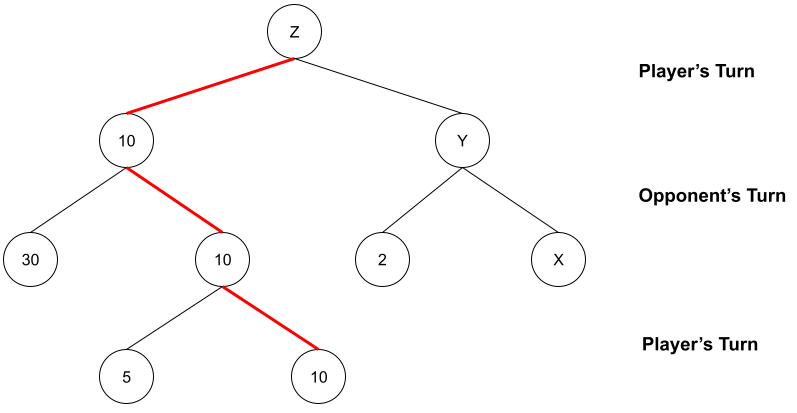
\includegraphics[width=\linewidth]{../img/Minimax2.png}
    \caption{Exemplary figure illustrating the alpha beta pruing for minimax algorithm}
    \label{fig:minimax2}
\end{figure}

Alpha-beta pruning is a another way to reduce the number of nodes that are evaluated by the minimax algorithm. In many cases, there may be the actions of the player in the search tree that can be evaluated worse than another action already evaluated. In such cases, where the better move or action has already been determined, it may not be useful to further evaluate the subsequent moves of the player and the opponent. Hence, the alpha-beta pruning moves on to another action instead of further evaluating the worse action.

As its name suggests, the alpha beta algorithm maintains two values, alpha and beta values. The alpha value stores the minimum score the player is assured to get while the beta value records the maximum score the opponent is assured to get. Whenever the evaluation of the minimum score of the player is higher than the maximum score after the subsequent move of the opponent (or in other words alpha > beta), the alpha-beta pruning algorithm stops evaluating the opponents position. This reduces the number of nodes in the search tree and hence reduces the complexity of the minimax algorithm.

In Figure \ref{fig:minimax2}, if the player determines that 
\begin{equation}
    Z = max (10, Y) = max (10,  min (2, X))
\end{equation}
, the value of X does not influence the value of $Y$ or $Z$ as $Y = min(2, X) \leq 2$ and hence $Z = max(10, \leq 2) = 10$. In this case, the player may not evaluate the branch $X$ or branch $Y$ further reducing the game tree and hence the computational complexity of the algorithm. 

\subsection{Parallel minimax}
Another way to improve the time complexity of the minimax algorithm is to parallelize the algorithm. The minimax algorithm involves in evaluating multiple nodes of the game tree. The way to parallelize such algorithm is to run different processes, in this case, evaluation of the position associated with different nodes, in different threads. This ensures that even though computational complexity may remain the same, the time complexity of the algorithm is distributed over multiple threads and possibly multiple processors.

For example, in Figure \ref{fig:minimax1}, the player can evaluate the branches with evaluation 10 and 2 in parallel reducing the time complexity of the algorithm.


The above defined methods to reduce the computational complexity of the minimax algorithm can be combined together. For example, the minimax algorithm can be depth limited and/or run with alpha-beta pruning and/or run in parallel.

\section{\ac{MCTS}}

\begin{figure}[!ht]
    \centering
    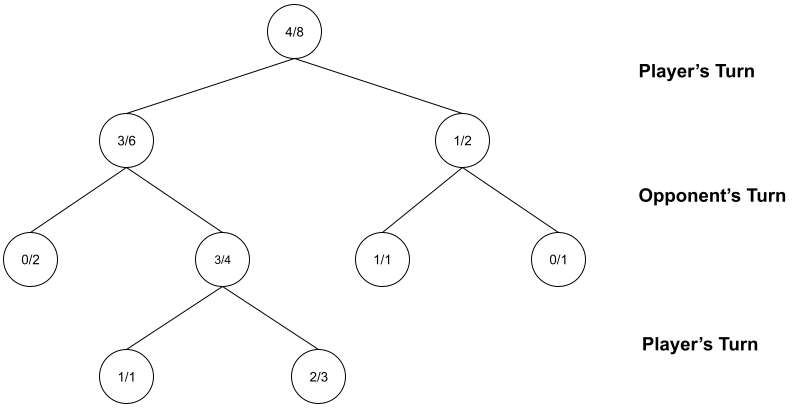
\includegraphics[width = \linewidth]{../img/MCTS1.png}
    \caption{Figure illustrating an iteration of the MCTS algorithm}
    \label{fig:MCTS1}
\end{figure}

\ac{MCTS} \cite{Coulom2006Efficient} is a heuristic tree search algorithm popular in decision-making processes, mostly popular in strategic games such as chess and Go to solve the game tree. This algorithm is mostly popular in scenarios where the game tree space is too large to traverse. One problem with the minimax algorithm is that it requires a robust and accurate evaluation function to evaluate a given position in the game. This problem can be even more relevant when the game tree space is too large making it difficult to find the evaluation of a position.

The basic idea of the \ac{MCTS} algorithm is that is narrows down on certain areas of the game tree, such that the exhaustive traversal and search of the tree is not required. The algorithm achieves this by taking random samples in the tree space and building a search tree based on it. For example, for a given position in tic-tac-toe, the \ac{MCTS} algorithm can be executed randomly a large number of times. Based on the statistics of the game wins and losses based on selection of certain moves, the weights are allocated to the children nodes in the graph.

An example of the \ac{MCTS} algorithm is presented in Figure \ref{fig:MCTS1}. The game is evaluated from the given position (e.g., the root node in the graph) for players and opponenent turns. The policy for the game can be random (e.g., determined by a random variable with certain distribution such as the uniform random distribution). Each node is labelled with a fraction where the denominator represents the total number of game runs through the node and the numerator represents the total number of wins for the player based on the game run through the node. For example, the game is simulated a total of 8 times in the example where the player wins 4 of the runs. The player wins 3/6 when taking an action while 1/2 when taking another action and so on.

The \ac{MCTS} algorithm builds upon the following framework:
\begin{enumerate}
    \item Selection: This step involves the algorithm choosing a move based on either a good move determined in previous iterations or a exploratory new move. In figure \ref{fig:MCTS1}, in the first player's turn, an action gives 3/6 chances of winning based on previous iterations whereas another gives 1/2 winning chances. The player selects a node that has highest possibility of winning, which in this case is equal. The player can also choose a new move that may be already explored to avoid not exploring further options.
    \item Expansion: This step involves the algorithm to add a new node to the game tree determined during the selection process. A node can simply be a valid move starting from the node from where no simulation step has been played out. In figure \ref{fig:MCTS2}, an unevaluated option (e.g., node inside the dotted box) is explored and simulated.
    \item Simulation: This step involves in playing out the game using policy. One of the policies can simply be a random policy (e.g., choosing a move based on certain distribution).
    \item Back propagation: Finally, based on the simulation step, this step involves in the algorithm updating the nodes. In figure \ref{fig:MCTS2}, the red arrows show the back propagation step as a result of exploration and simulation step where the probabilities or the weights of the nodes are updated as a result of exploration and simulation steps.
\end{enumerate}

\begin{figure}[!ht]
    \centering
    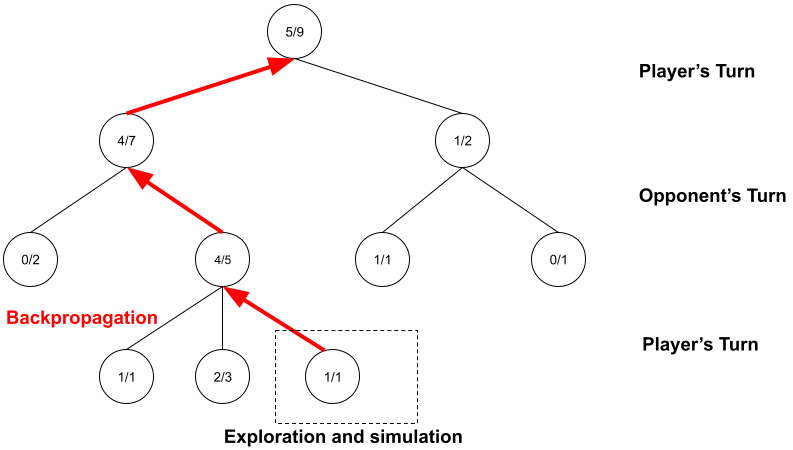
\includegraphics[width=\linewidth]{../img/MCTS2.png}
    \caption{Figure illustrating steps 2, 3, and 4 of the MCTS algorithm}
    \label{fig:MCTS2}
\end{figure}

The advantage of \ac{MCTS} algorithm over the minimax algorithm is that the \ac{MCTS} algorithm does not require any evaluation function as the weights are determined based on multiple simulation runs. On the contrary, the \ac{MCTS} algorithm requires multiple runs through the game to determine the weights.